% !TEX root = ../main.tex
\chapter{Empirical Context and Data} \label{chap:data_empirics}

This chapter introduces the empirical context and data used in our analysis. We begin by introducing our source of exogenous variation in remittance flows, Hurricane Ian. First, we document the hurricane's impact on Florida's remittance outflows as well as sectors with high Mexican immigrant employment. Next, we explain the data sources and the methodology we use to construct our treatment measure, which differentiates Mexican municipalities by how exposed they are to the shock. Finally, we present a validation exercise, justifying the choice of our constructed treatment variable as a proxy for the Mexican migrant population in the United States.

\section{The Natural Experiment: Hurricane Ian (2022)}

Hurricane Ian struck the southwestern coast of Florida on September 28, 2022, with peak sustained winds of 140 kt (around 260 kph) \parencite{nhc_ian_2026}. Ian caused an estimated US\$\,112.9 billion in total damage in the United States, of which US\$\,109.5 billion occurred in Florida alone, making it simultaneously the costliest hurricane in Florida's history and the third-costliest in US history. In Lee County alone, at least 52,514 structures were impacted, of which 5,369 were completely destroyed \parencite{nhc_ian_2026}.

Beyond its aggregate toll, Ian's destruction fell on sectors that employ a large share of Mexican migrants. Construction is the single largest sector of employment for Mexican-born workers in Florida, at roughly 28\% of all those employed, and the four sectors most exposed to the storm together account for over 50\% of Mexican workers. Within them, construction makes up 52\%, agriculture 17\%, landscaping 16\%, and hospitality 15\%.\footnote{Calculated using IPUMS USA, ACS 1-year samples 2021--2024, employed Mexican-born residents of Florida. The full industry composition and the within-sector shares are reported in the online appendix.} Construction is therefore both the main source of work for Mexican workers and the channel where Ian's damage translates most directly into lost employment, and later into reconstruction demand. 

\autoref{fig:construction-origin} indexes Florida construction employment to 2021 by workers' region of birth. The Mexican-born series diverges from the US-born and other foreign-born series after Ian, falling to roughly 92\% of its 2021 level in 2023 before rebounding to about 117\% in 2024. The US-born series drifts upward throughout, which suggests the disruption was specific to migrant labor rather than to construction as a whole. \autoref{fig:construction-citizenship} shows that this movement is carried by non-citizens, who make up the large majority of Mexican-born construction workers in the state and absorb both the 2023 dip and the 2024 rebound. Non-citizens are also the group most reliant on remittances as a financial link to their origin households \parencite{chicago_fed_2002}. The descriptive evidence thus indicates that Ian affected workers whose earnings finance remittances to Mexico, which motivates the migrant income channel we examine in the remainder of the paper.
\begin{figure}[H]
    \centering
    \begin{subfigure}{0.48\textwidth}
        \centering
        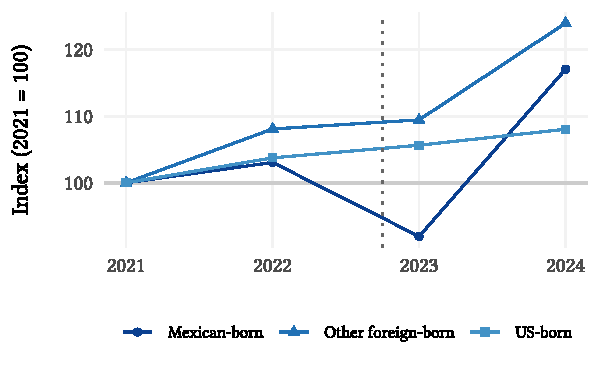
\includegraphics[width=\textwidth]{../figures-tables/descriptive/FL_construction_indexed_by_origin.pdf}
        \caption{Construction employment by region of birth, indexed to 2021}
        \label{fig:construction-origin}
    \end{subfigure}
    \hfill
    \begin{subfigure}{0.48\textwidth}
        \centering
        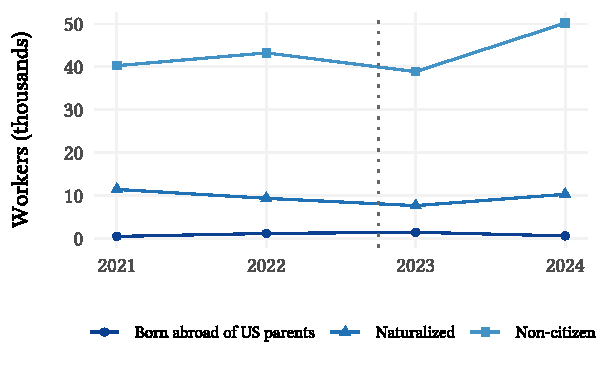
\includegraphics[width=\textwidth]{../figures-tables/descriptive/mexican_construction_citizenship.pdf}
        \caption{Mexican-born construction workers by citizenship status}
        \label{fig:construction-citizenship}
    \end{subfigure}
\ 
    \caption{Mexican-born construction employment in Florida around Hurricane Ian. Source: IPUMS USA, ACS 1-year samples 2021--2024; employed Florida construction workers. Dotted line marks Hurricane Ian (2022Q4).}
    \label{fig:construction}
\end{figure}
Crucially for our identification strategy, Hurricane Ian did not affect Mexico. The storm originated in the Caribbean, made landfall in Cuba and Florida, and dissipated over the Atlantic after a final less impactful landfall in South Carolina \parencite{nhc_ian_2026}. Therefore, the shock is spatially clean, allowing us to better isolate the transmission mechanism through the remittance channel. In the language of the model proposed in Chapter \ref{chap:structural_model}, Hurricane Ian is the negative shock to migrants' economic resources, Florida is the affected destination, and Mexican municipalities differ in their pre-existing exposure to Florida through migration networks.

To motivate the analysis, \autoref{fig:florida-outflows} presents the evolution of remittance outflows from Florida to Mexico using data from Banxico series CE168 \parencite{banxico_ce168}. A sharp decline in remittance outflows can be observed in the quarter immediately following Hurricane Ian, with flows falling by approximately 40\% relative to the previous quarter. This pronounced contraction suggests that the hurricane generated a substantial disruption in remittance activity from Florida to Mexico, thereby providing a strong motivation for examining its effects on Mexican municipalities' remittance inflows.\footnote{Florida outflows are plotted against the average outflows of all other U.S. states. Because the comparison series is constructed as an average, potential opposite shocks affecting individual states during the Hurricane Ian period may be attenuated. Nevertheless, the purpose of the figure is simply to illustrate the magnitude of the decline observed in Florida.}
\begin{figure}[H]
    \centering
    \IfFileExists{../figures-tables/state-outflows/total_remittance_outflows.pdf}{%
        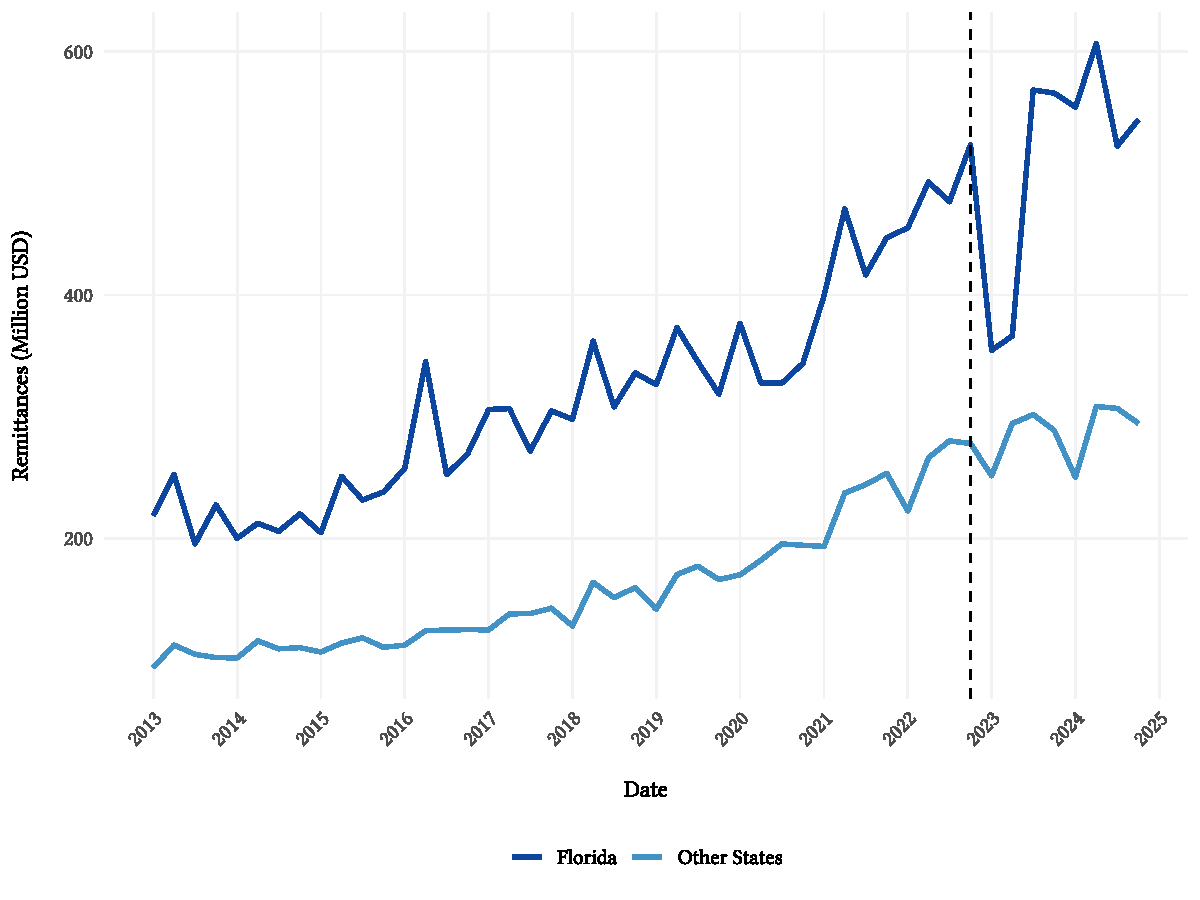
\includegraphics[width=0.85\textwidth]{../figures-tables/state-outflows/total_remittance_outflows.pdf}%
    }{%
        \fbox{\parbox{0.85\textwidth}{\centering\vspace{2cm}[Figure pending]\vspace{2cm}}}%
    }
    \caption{Remittance outflows from Florida to Mexico, in millions of US dollars. The vertical dashed line indicates the quarter of Hurricane Ian (Q4 2022).}
    \caption*{Source: Authors' own elaboration based on Banxico SIE data.}
    \vspace{-16pt}
    \label{fig:florida-outflows}
\end{figure}

\section{Data Sources}

Given that bilateral remittance flows between US States and Mexican municipalities are not publicly available, we base our estimation strategy on multiple data sources. The source of remittance data is Banco de México (Banxico), through the datasets provided by its Sistema de Información Económica (SIE). Specifically, series CE166 records remittance inflows received by each Mexican municipality. This series is available at quarterly frequency, from Q1 2013 to Q1 2026 and represents our outcome variable \parencite{banxico_ce166}. To capture the Mexican migration network, we utilize administrative records from the Matricula Consular de Alta Seguridad (MCAS) program, managed by the Instituto de los Mexicanos en el Exterior (IME) \parencite{ime_estadisticas_2026}. The publicly available version of this dataset provides a comprehensive registry of consular identification cards issued to Mexican nationals residing in the United States each year, from 2010 to 2024. While the MCAS does not constitute an exhaustive census of all migrants, it represents a robust proxy for the spatial distribution of Mexican migrants in the United States. In particular, it is highly representative of undocumented and recently arrived migrants, who face the strongest incentives to obtain consular identification \parencite{caballero_cadena_kovak_2018}. 

\section{Migration Networks Construction} \label{sec:migration-network-construction}

To build our treatment measure, we construct a migration-based matrix using annual MCAS data from 2014 to 2021. Because these records capture new consular issuances rather than the complete stock of the remitting population, which also includes previously arrived migrants, we rely on the assumption of persistence of migration patterns over time \parencite{card2001, munshi2003}. Additionally, we rely on the fact that there is no significant internal mobility within Mexico, allowing us to link remittance receiving municipalities to the migrants' origin villages. This is supported by the literature, showing that internal mobility has decreased over the last few decades \parencite{gordillo2017movilidad,partida2014migracion}. 

\par

To mitigate the volatility of yearly migration fluctuation and construct a robust proxy for the long-term spatial distribution of Mexican migrants, we compute the average of the migration matrices across all years. Formally, we define $MCAS_{ms}$ as the average annual count of MCAS issuances to migrants from Mexican municipality $m$ residing in U.S. state $s$. For each Mexican municipality, we calculate the average migration network share, $w_{ms}$, which represents the proportion of municipality $m$'s total US migrant population that resides in state $s$. This is calculated as the ratio of $MCAS_{ms}$ to the total number of MCAS issuances for migrants from municipality $m$ across all U.S. states $S$:
\begin{equation} \label{eq:weights}
w_{ms} = \frac{MCAS_{ms}}{\sum_{s=1}^{S} MCAS_{ms}}
\end{equation}

By construction, the sum of $w_{ms}$ across all U.S. states for a given Mexican municipality $m$ equals 1, and the value of $w_{ms}$ for a specific state $s$ reflects the relative importance of that state as a destination for migrants from municipality $m$, which in turn is a proxy for the exposure of municipality $m$ to shocks occurring in state $s$. 

\section{Persistence Assumption and Validation}

The validity of this estimation relies on the assumption of temporal persistence of migration flows, implying that the distribution of migrants recorded in the MCAS data is representative of the active remitting population. The stability of migration patterns over time is well-documented in the literature, with studies showing that existing migration networks tend to dictate future migration patterns, creating persistent flows between specific origin and destination pairs \parencite{card2001, munshi2003}. To verify this assumption within our specific sample period, we conduct a validation exercise using MCAS data. Figure \ref{fig:persistence} computes the Pearson correlation of our constructed weighting matrices across years. As observed, when taking any year from 2014 onward as the base year, the correlation with subsequent years is consistently above 0.90. 
\begin{figure}[H]
    \centering
    \IfFileExists{../figures-tables/municipality-inflows/network_persistence_all_base_years.pdf}{%
        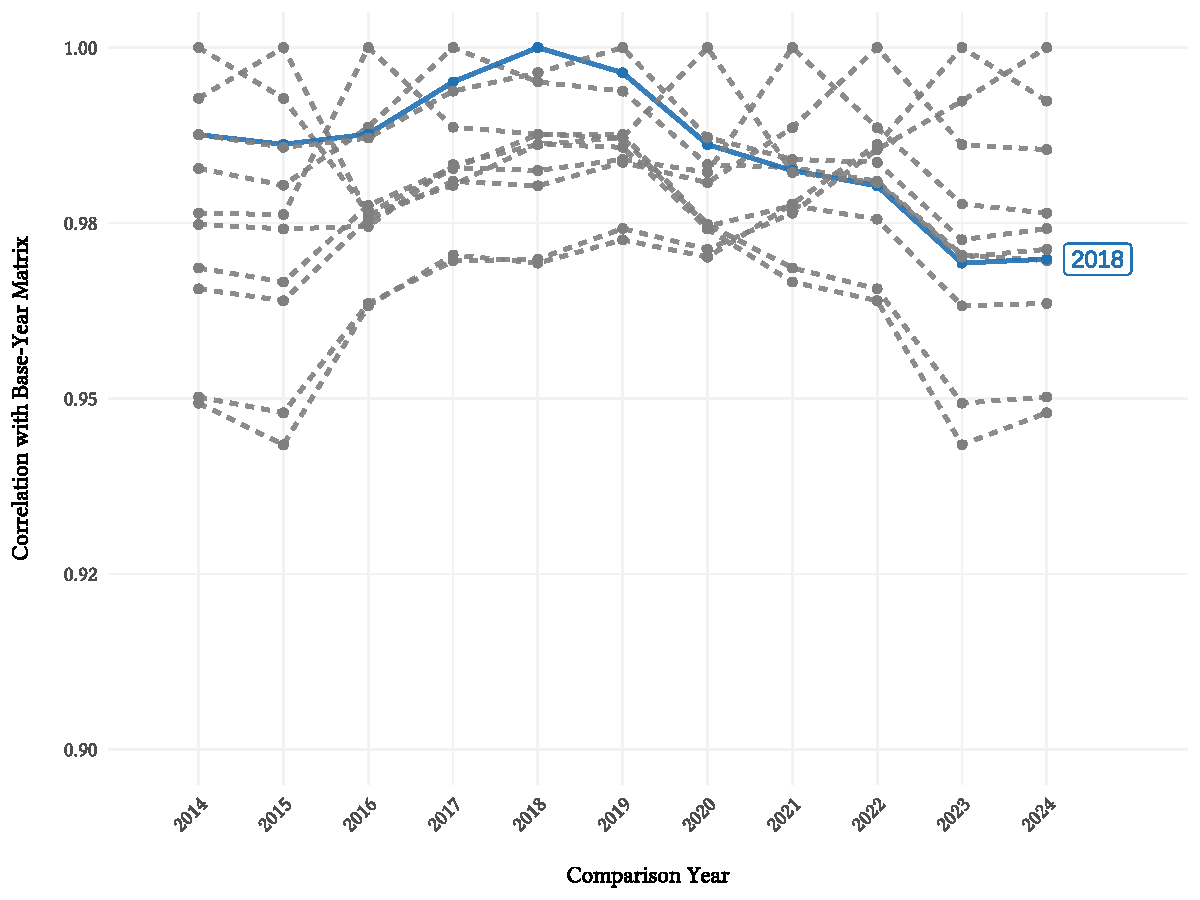
\includegraphics[width=0.85\textwidth]{../figures-tables/municipality-inflows/network_persistence_all_base_years.pdf}%
    }{%
        \fbox{\parbox{0.85\textwidth}{\centering\vspace{2cm}[Figure pending]\vspace{2cm}}}%
    }
    \caption{Correlation of MCAS-based weighting matrices across years. Each point represents the correlation coefficient between the weighting matrix of the base year and the weighting matrix of the comparison year (2018 as base year is highlighted in blue for demonstration purposes).}
    \caption*{Source: Authors' own elaboration based on MCAS data.}
    \vspace{-16pt}
    \label{fig:persistence}
\end{figure}

This high degree of correlation suggests that the spatial distribution of Mexican migrants across U.S. states has remained highly stable over time, lending credibility to our use of an averaged weighting matrix for estimating bilateral remittance flows. Given that Hurricane Ian hit florida in Q4 2022 and the MCAS data for Florida in 2013 is missing, to construct our treatment variable we use the average of the weighting matrices from 2014 to 2021, which are all highly correlated with each other, and avoid any endogeneity in the treatment caused by the shock.